\documentclass{article}

\usepackage{template}



\usepackage[utf8]{inputenc} % allow utf-8 input
\usepackage[T1]{fontenc}    % use 8-bit T1 fonts
\usepackage{hyperref}       % hyperlinks
\usepackage{url}            % simple URL typesetting
\usepackage{booktabs}       % professional-quality tables
\usepackage{amsfonts}       % blackboard math symbols
\usepackage{nicefrac}       % compact symbols for 1/2, etc.
\usepackage{microtype}      % microtypography
\usepackage{xcolor}         % colors
\usepackage{graphicx}
\graphicspath{ {./imagenes/} }

\title{Pre TP1: Data Mining en Ciencia y Tecnología}

\author{%
  José Saint Germain\\
  \texttt{josesg998@gmail.com} \\
}

\begin{document}

\maketitle

\section{Procesamiento de imágenes}

{\emph Cargar el dataset de imágenes y sus respectivas etiquetas. Es importante asegurarse que las 
imágenes sean comparables en color, valor, rango y tamaño.

Explorar y graficar los subconjuntos de imágenes que representan flores de la misma
especie.}

En el siguiente gráfico, se tomó una muestra de cuatro flores por especie:

\begin{figure}[h!]
  \centering  
  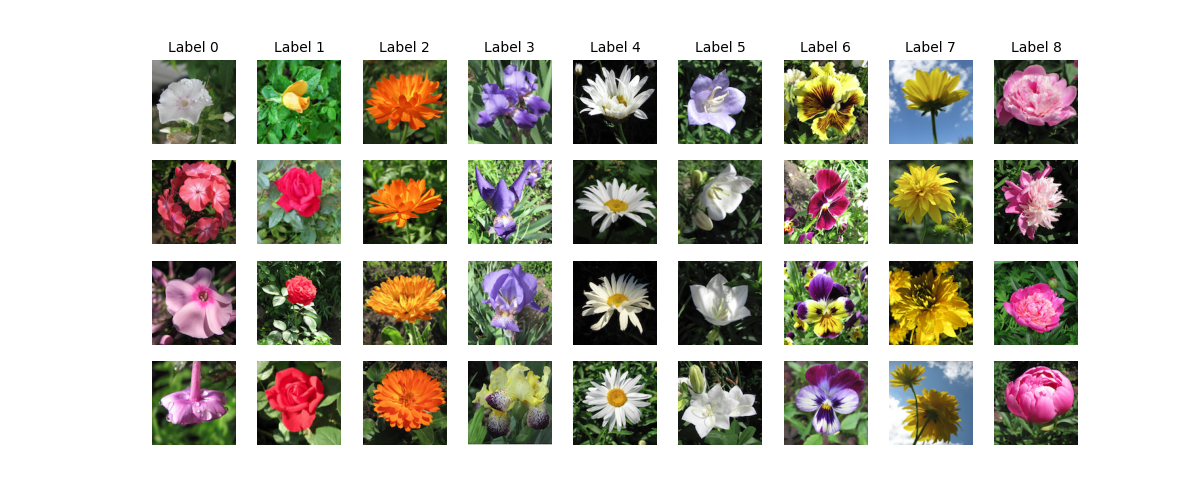
\includegraphics[width=1\textwidth]{1_ejemplos_flores.png}
  \caption{Exploración de especies de flores}
\end{figure}

En cada una de ellas se pueden apreciar determinadas características comunes que permiten diferenciarlas de las otras 8, en especial el color de sus pétalos.

\section{Manipulación de datos}

\subsection{Cambio de brillo}

{\emph Cambiar la intensidad de una de las imágenes en escala de grises, transformarla en una imagen con mucho y otra con poco brillo.}

\begin{figure}[h!]
  \centering    
  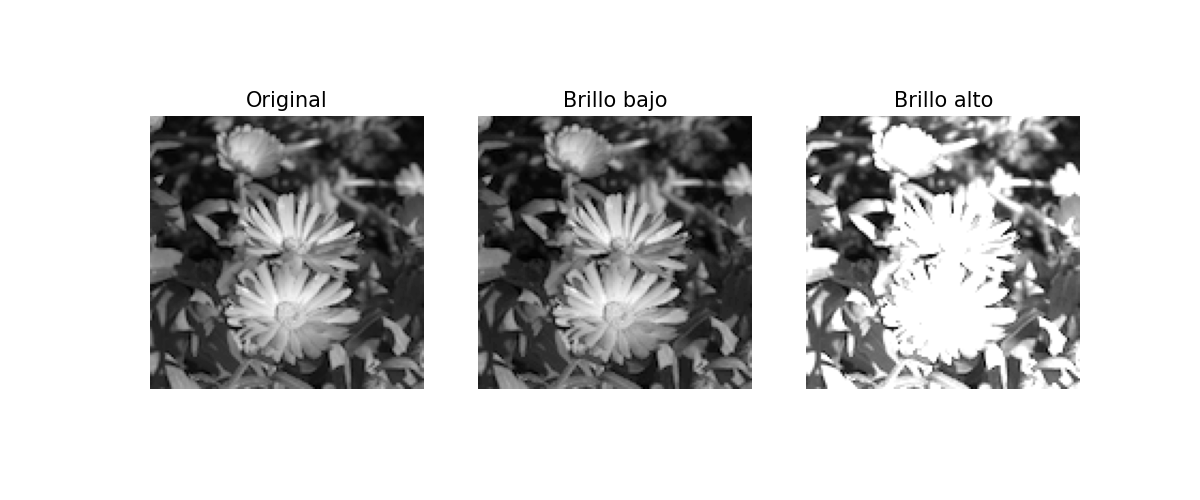
\includegraphics[width=.75\textwidth]{2_brillo.png}
  \caption{Ajuste de brillo}
\end{figure}
\pagebreak
\subsection{Imagen en blanco y negro}

{\emph Convertir una de las imágenes a blanco y negro (binario). ¿Es la única manera? Si existen otras transformaciones mostrar más de una conversión}

\begin{figure}[h!]
  \centering    
  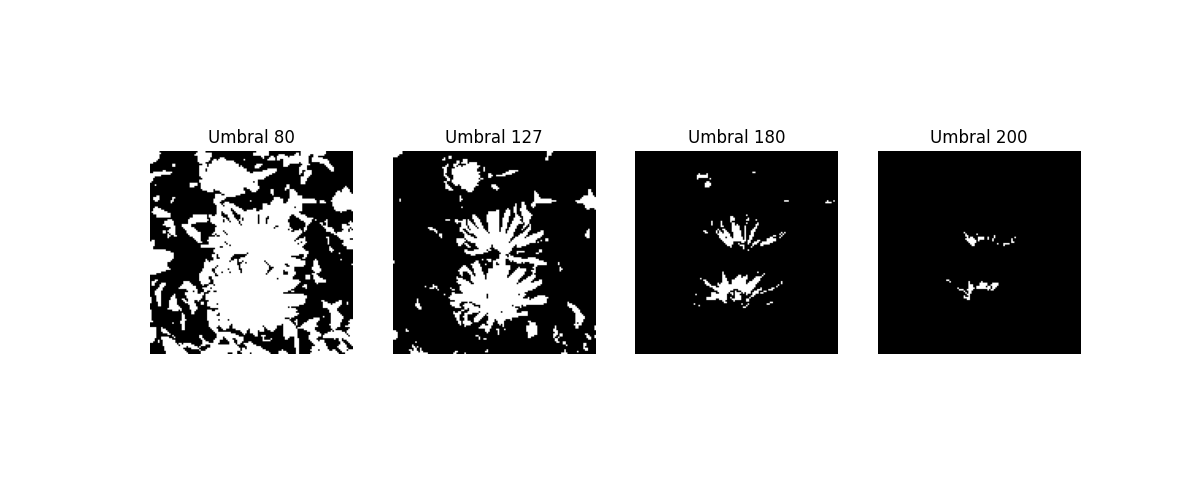
\includegraphics[width=.75 \textwidth]{3_binario.png}
  \caption{Imágenes binarias con disintos umbrales}
\end{figure}

Para pasar una imagen a binaria, es necesario establecer un umbral. De esa manera, cualquier pixel que supere ese umbral será blanco y cualquier pixel que esté por
debajo será negro. A medida que se aumente el umbral, como se ve en las imágenes, una mayor proporción de los píxeles pasarán a ser negros.

\subsection{Imagen recortada}
\label{others}

{\emph Recortar una parte significativa de la imagen, quedándose sólo con el círculo central de la misma.}

\begin{figure}[h!]
  \centering    
  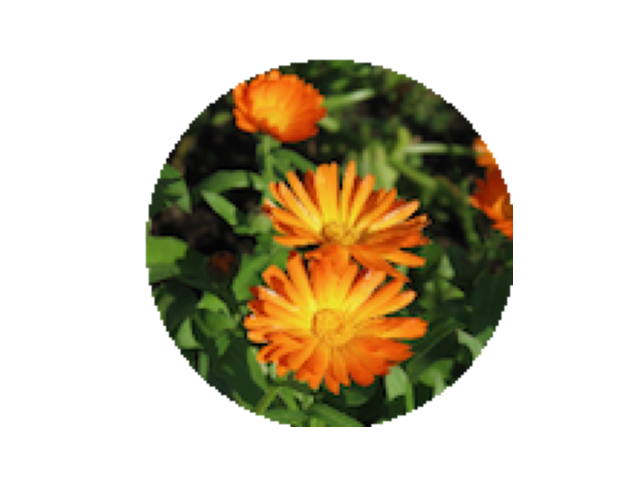
\includegraphics[width=.3\textwidth]{4_recortado.png}
  \caption{Recorte de imagen}
\end{figure}
\subsection{Imágenes mezcladas}

{\emph Generar dos imágenes random: una imagen mezclando los pixels y otra mezclando
partes de diferentes imágenes.}

\begin{figure}[h!]
  \centering    
  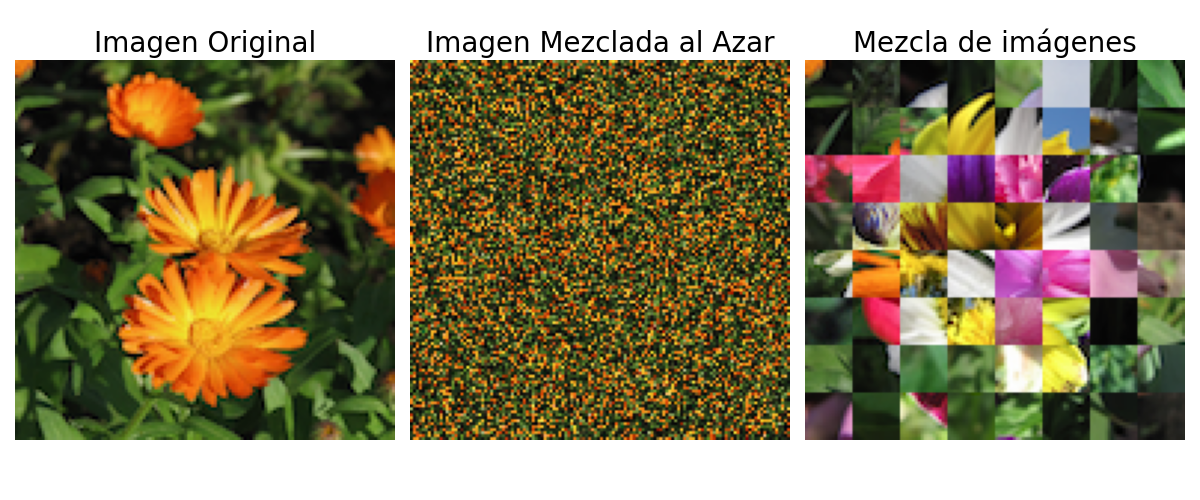
\includegraphics[width=.75\textwidth]{5_mezcla.png}
  \caption{Imagenes con píxeles mezclados e intercambiados}
\end{figure}

Para ambos casos, se puede alterar el tamaño de la porción de las imágenes, por lo que se podría mezclar cada pixel, o bien utilizar cuadrados más grandes como en la imágen con píxeles de varias flores.

\subsection{Filtros de imagen}

{\emph Aplicar dos tipos diferentes de filtros sobre una imagen, 
explique en qué casos conviene usar cada uno.}
\begin{figure}[h!]
  \centering    
  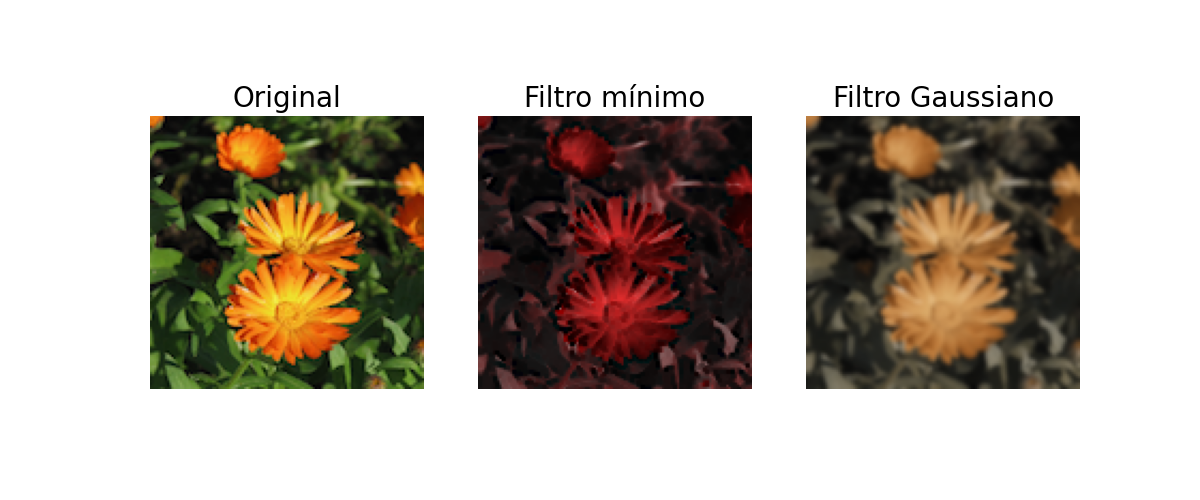
\includegraphics[width=1\textwidth]{6_filtro.png}
  \caption{Imagenes con filtros}
\end{figure}

El filtro mínimo toma una porción de píxeles (en este caso, de tamaño 2) y 
le aplica a todos el valor del píxel mínimo. Se utiliza para remover 
outliers positivos, es decir píxeles de colores claros.

El filtro gaussiano tiene un uso similar al mean filter, con la
diferencia de que el primero tiene en cuenta la distancia de los 
píxeles a los que se les aplica el filtro. De esa manera, los píxeles
más cercanos al centro del conjunto de píxeles (en este caso se seleccionó un
desvío estándar de 1) tienen mayor peso que los lejanos. Se suele preferir
frente al mean filter cuando se quiere suavizar la imagen pero sin transiciones
fuertes entre los píxeles.

\subsection{Imágenes promedio}

{\emph Calcular imagen promedio global y el promedio entre las distintas especies. ¿Se pueden
distinguir los promedios? ¿Cómo quedan los promedios si consideran las imágenes en
blanco y negro?}

\begin{figure}[h!]
  \centering    
  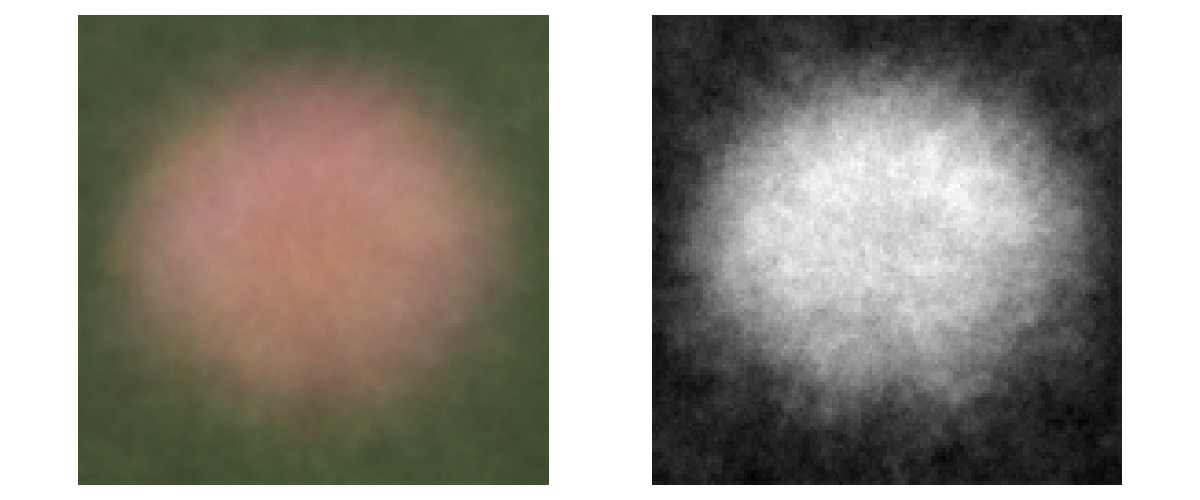
\includegraphics[width=.4\textwidth]{7_1_promedio.png}
  \caption{Imagenes promedio color y blanco y negro}
\end{figure}


\begin{figure}[h]
  \centering    
  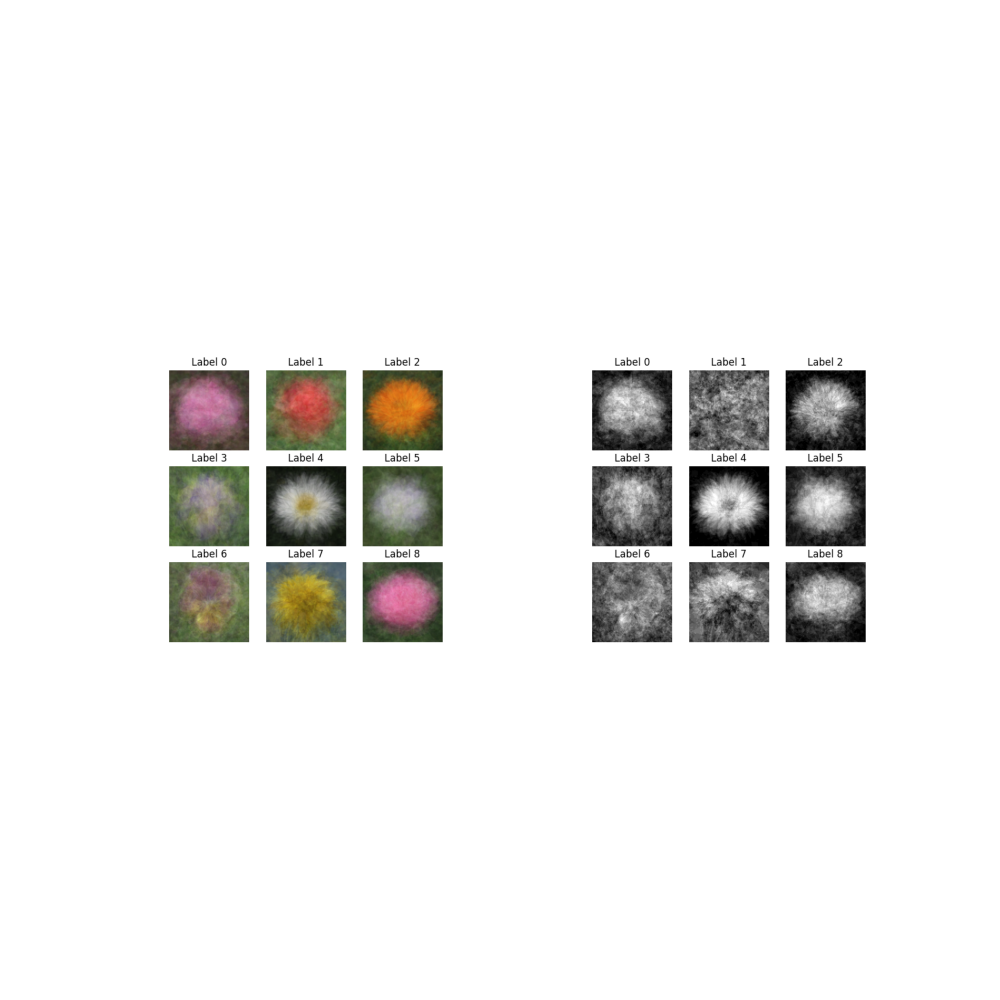
\includegraphics[width=1\textwidth]{7_4_promedio_especies_ambos.png}
  \caption{Imagenes promedio por especie}
\end{figure}


%\begin{figure}[h!]
%  \centering    
%  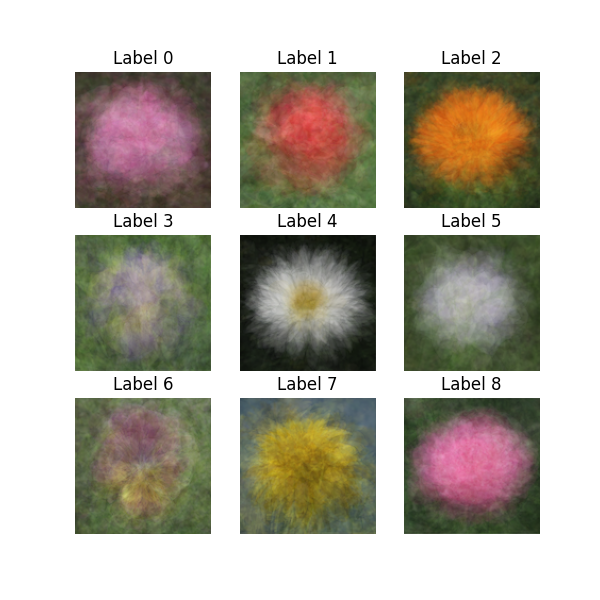
\includegraphics[width=.6\textwidth]{7_2_promedio_especies_color.png}
%  \caption{Imagenes promedio color}
%\end{figure}

%\begin{figure}[h!]
%  \centering    
%  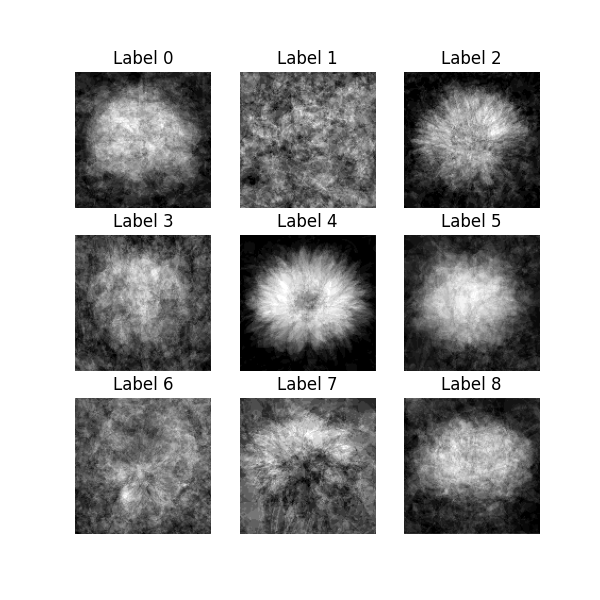
\includegraphics[width=.6\textwidth]{7_3_promedio_especies_bn.png}
%  \caption{Imagenes promedio blanco y negro}
%\end{figure}
Analizando todos los archivos noté que la imagen '00218.png' tiene una resolución mayor a la del resto, lo cual puede dificultar algunos análisis como el cálculo de la imagen promedio. Por lo tanto, se decidió quitar la imagen del análisis.

Con respecto a la imagen promedio, tanto a color como en blanco y negro, se pueden extraer dos características: que las flores comparten una forma redonda, y que cuentan con un fondo verde.

Las imágenes promedio en color se pueden distinguir con facilidad. Incluso, en el caso de la especie 4, permite identificar de forma bastante precisa el círculo central amarillo. En el resto, se puede apreciar el rango de color en el que se manejan sus pétalos. Las imágenes en blanco y negro, en cambio, dificultan identificar diferencias
entre especies, a excepción de la especie 4. En la especie 1 ni siquiera se puede identificar la flor con respecto al fondo.

\section{Búsqueda de features}

{\emph Analizar las distribuciones de valores de pixels por cada especie. ¿Se puede distinguir
una especie en algún rango de color?}

% \begin{figure}[h!]
%   \centering    
%   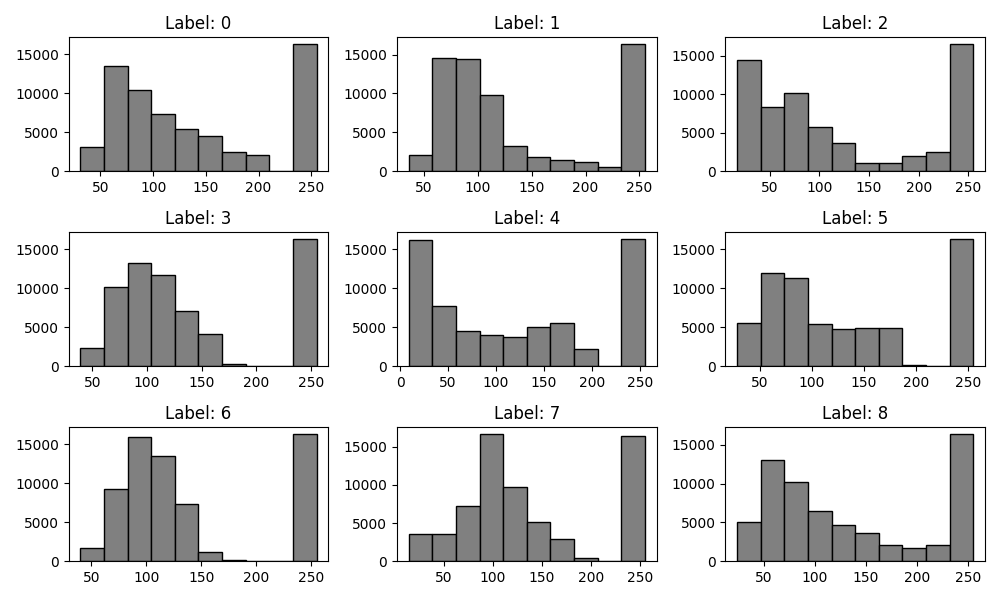
\includegraphics[width=1\textwidth]{8_2_pixeles_especies_byn.png}
%   \caption{Distribución de pixeles por especie}
% \end{figure}

\begin{figure}[h!]
  \centering    
  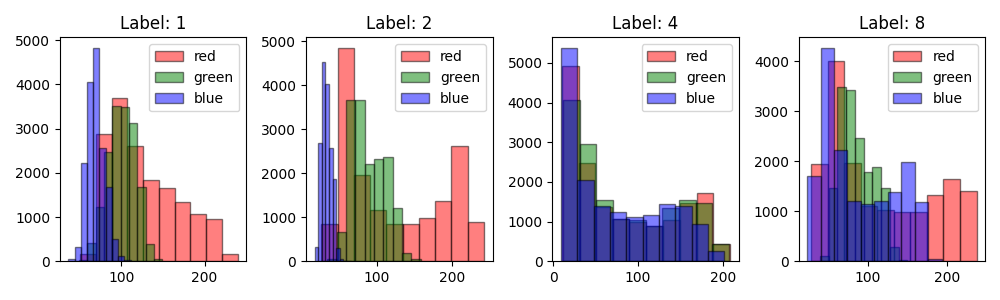
\includegraphics[width=1\textwidth]{8_3_pixeles_especies_color_muestra.png}
  \caption{Distribución de pixeles de color por especie}
\end{figure}

Para este análisis, es muy útil referenciarse con las imágenes promedio.
Por ejemplo, las especies 1, 2 y 8 contienen una gran cantidad de píxeles
rojos de alto valor, lo cual se evidencia en que el color de sus pétalos son cercanos al rojo. Otra especie a destacar es la 4, puesto que la distribución de los tres colores es casi idéntico, expresándose en sus pétalos blancos.

\subsection{Análisis de componentes principales}

{\emph Realizar una inspección de las componentes principales del dataset y analizar si se
pueden identificar las especies en esta representación.}

Una vez escaladas las variables y obtenido los componentes principales, se midió y graficó la varianza explicada acumulada de cada componente. Como se ve en el gráfico de la
izquierda, los primeros 2 componentes explican el 20 por ciento de la varianza,
lo cual es un valor bastante bajo para realizar un análisis significativo.
Adicionalmente,  si quisiéramos explicar al menos el 70 por ciento de la varianza,
necesitaríamos un poco menos de 50 componentes.

Esta conclusión se refuerza con el gráfico de la derecha, en donde se utilizan los primeros dos componentes y se colorean los puntos con la especie correspondiente.
Como se puede apreciar, no se puede distinguir ningún grupo de puntos de un color particular.

\begin{figure}[h!]
  \centering    
  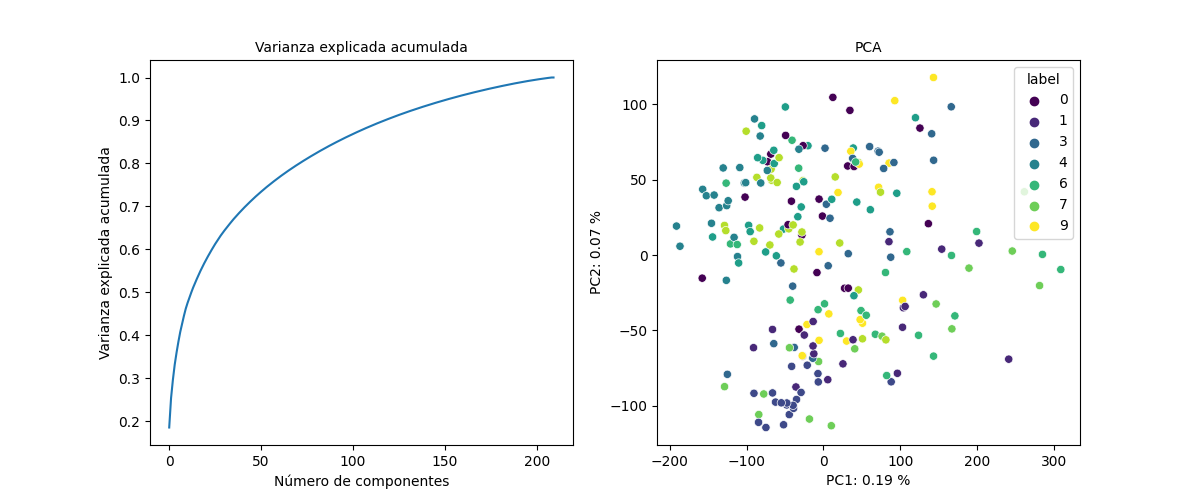
\includegraphics[width=.9\textwidth]{9_1_pca.png}
  \caption{Análisis de componentes principales}
\end{figure}

%%%%%%%%%%%%%%%%%%%%%%%%%%%%%%%%%%%%%%%%%%%%%%%%%%%%%%%%%%%%


\end{document}